\subsection{External interface requirements}
\subsubsection{User interface}

\begin{figure}[!h]
	\centering
	\begin{minipage}[b]{0.65\textwidth}
		\makebox[\textwidth][c]{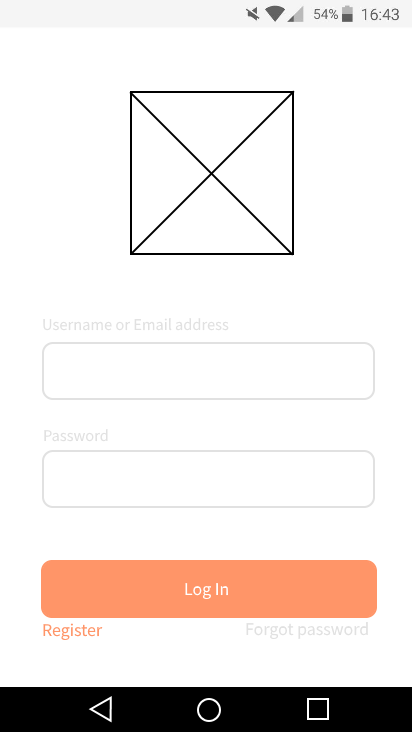
\includegraphics[width=0.50\textwidth]{Images/Mockup/LogPage.png}}%
		\caption{Login page}
	\end{minipage}
	\begin{minipage}[b]{0.65\textwidth}
		\makebox[\textwidth][c]{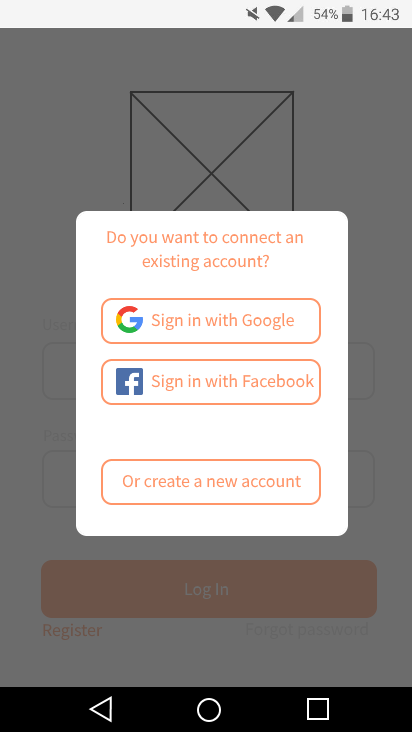
\includegraphics[width=0.50\textwidth]{Images/Mockup/GoogleConnectionPopup.png}}%
		\caption{Connection of an existent account}
	\end{minipage}
\end{figure}
\clearpage
\begin{figure}[!h]
	\centering
	\begin{minipage}[b]{0.65\textwidth}
		\makebox[\textwidth][c]{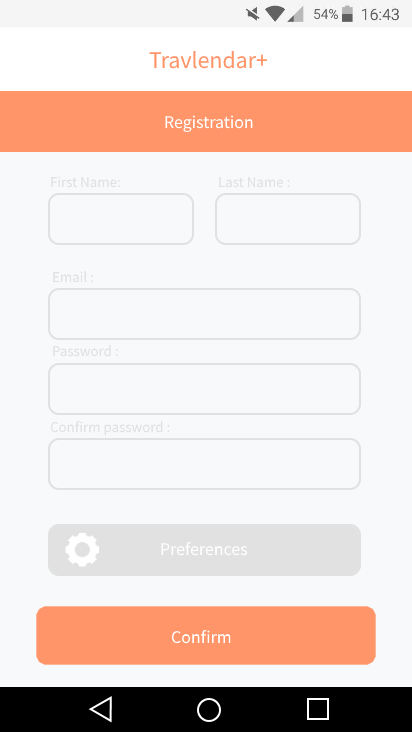
\includegraphics[width=0.50\textwidth]{Images/Mockup/RegistrationForm.png}}%
		\caption{Registration form}
	\end{minipage}
	\begin{minipage}[b]{0.65\textwidth}
		\makebox[\textwidth][c]{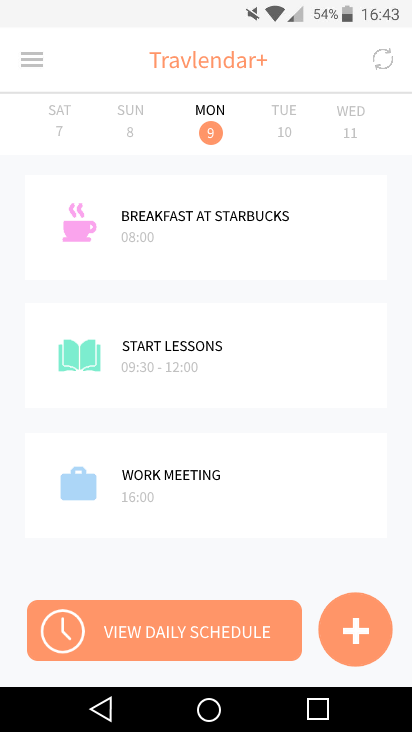
\includegraphics[width=0.50\textwidth]{Images/Mockup/Base.png}}%
		\caption{Daily view of calendar}
	\end{minipage}
\end{figure}
\clearpage
\begin{figure}[!h]
	\centering
	\begin{minipage}[b]{0.65\textwidth}
		\makebox[\textwidth][c]{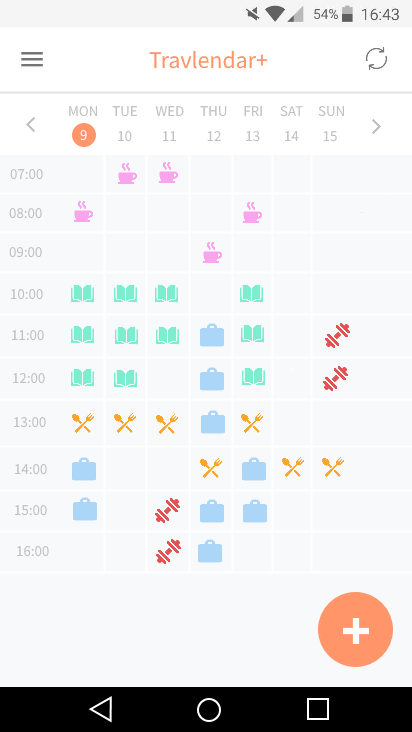
\includegraphics[width=0.50\textwidth]{Images/Mockup/Base3.png}}%
		\caption{Weekly view of calendar}
	\end{minipage}
	\begin{minipage}[b]{0.65\textwidth}
		\makebox[\textwidth][c]{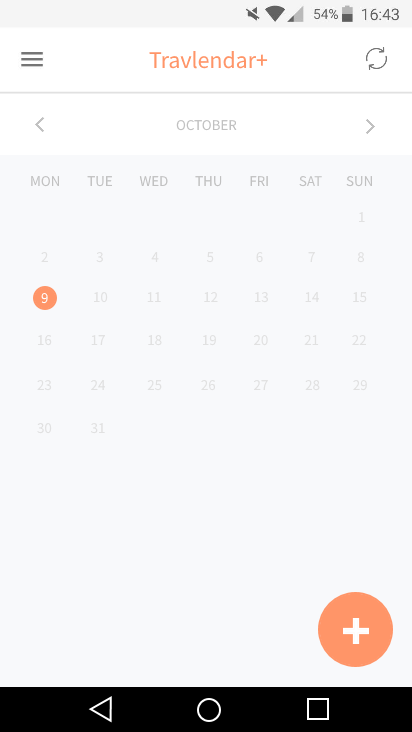
\includegraphics[width=0.50\textwidth]{Images/Mockup/Base2.png}}%
		\caption{Monthly view of calendar}
	\end{minipage}
\end{figure}
\clearpage
\begin{figure}[!h]
	\centering
	\begin{minipage}[b]{0.65\textwidth}
		\makebox[\textwidth][c]{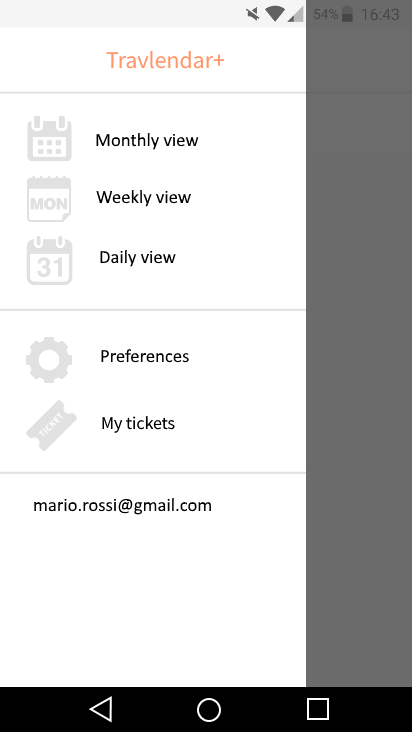
\includegraphics[width=0.50\textwidth]{Images/Mockup/LeftPanel.png}}%
		\caption{Menu}
	\end{minipage}
	\begin{minipage}[b]{0.65\textwidth}
		\makebox[\textwidth][c]{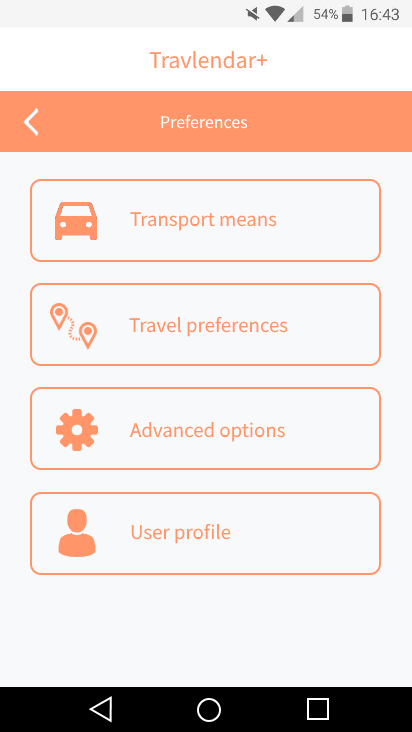
\includegraphics[width=0.50\textwidth]{Images/Mockup/PreferencesManager.png}}%
		\caption{Preferences menu}
	\end{minipage}
\end{figure}
\clearpage
\begin{figure}[!h]
	\centering
	\begin{minipage}[b]{0.65\textwidth}
		\makebox[\textwidth][c]{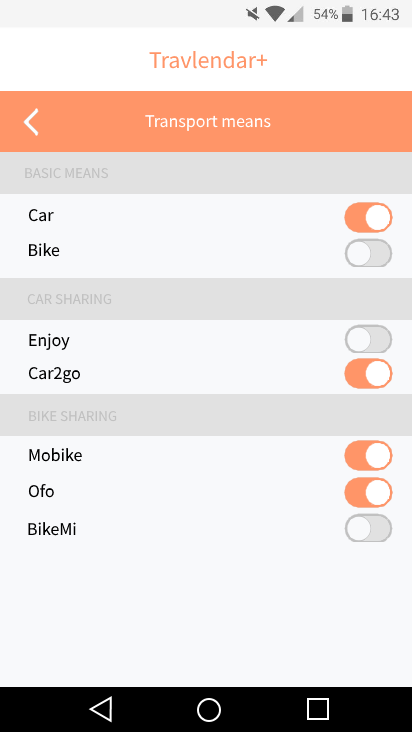
\includegraphics[width=0.50\textwidth]{Images/Mockup/transportMeansOpt.png}}%
		\caption{Transport means settings}
	\end{minipage}
	\begin{minipage}[b]{0.65\textwidth}
		\makebox[\textwidth][c]{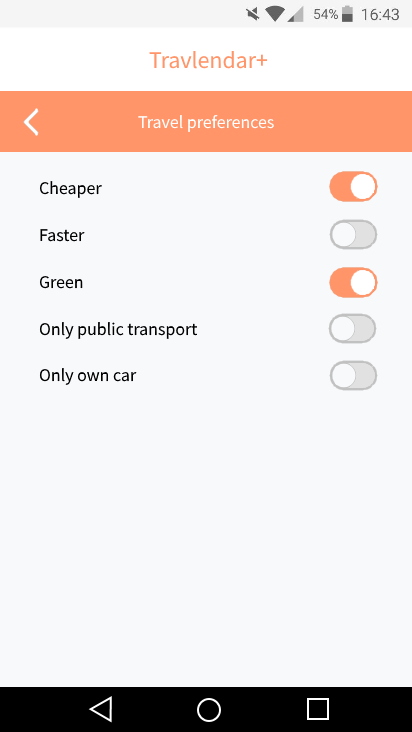
\includegraphics[width=0.50\textwidth]{Images/Mockup/TravelPreferences.png}}%
		\caption{Travel preferences}
	\end{minipage}
\end{figure}
\clearpage
\begin{figure}[!h]
	\centering
	\begin{minipage}[b]{0.65\textwidth}
		\makebox[\textwidth][c]{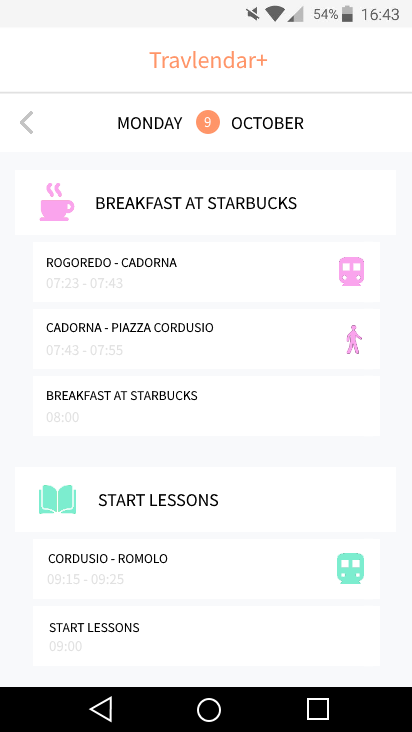
\includegraphics[width=0.50\textwidth]{Images/Mockup/DailySchedule.png}}%
		\caption{Daily schedule}
	\end{minipage}
	\begin{minipage}[b]{0.65\textwidth}
		\makebox[\textwidth][c]{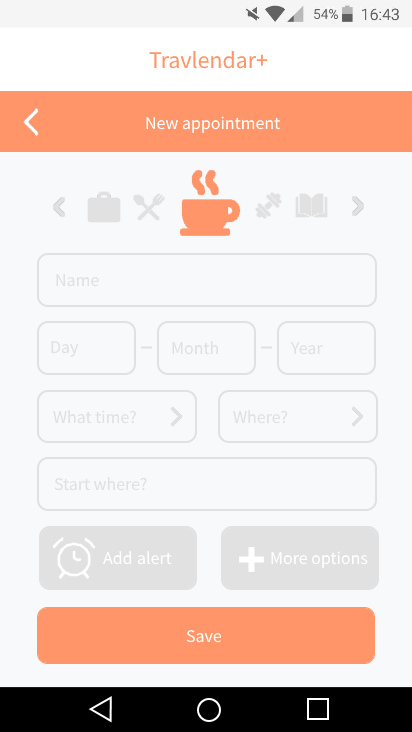
\includegraphics[width=0.50\textwidth]{Images/Mockup/EventCreator.png}}%
		\caption{New appointment}
	\end{minipage}
\end{figure}
\clearpage
\begin{figure}[!h]
	\centering
	\begin{minipage}[b]{0.65\textwidth}
		\makebox[\textwidth][c]{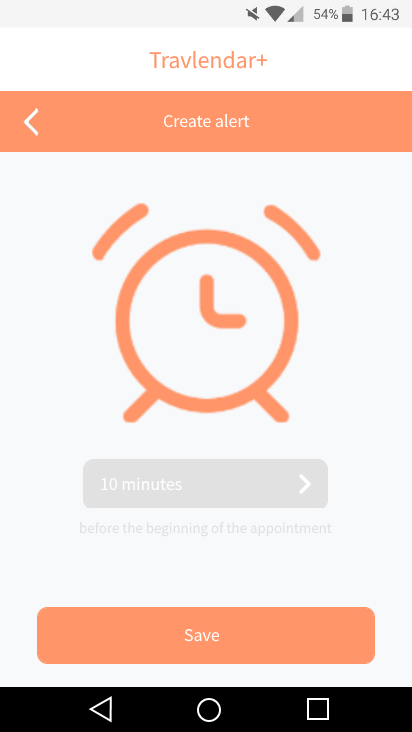
\includegraphics[width=0.50\textwidth]{Images/Mockup/AlarmCreator.png}}%
		\caption{New alert}
	\end{minipage}
	\begin{minipage}[b]{0.65\textwidth}
		\makebox[\textwidth][c]{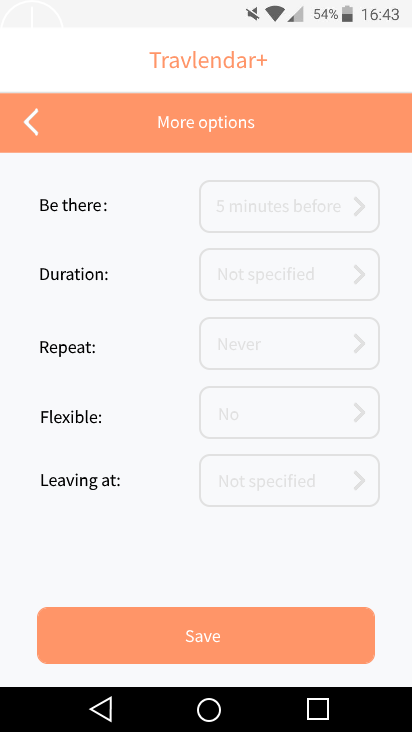
\includegraphics[width=0.50\textwidth]{Images/Mockup/OptionPanel.png}}%
		\caption{appointment options}
	\end{minipage}
\end{figure}
\clearpage
\begin{figure}[!h]
	\centering
	\begin{minipage}[b]{0.65\textwidth}
		\makebox[\textwidth][c]{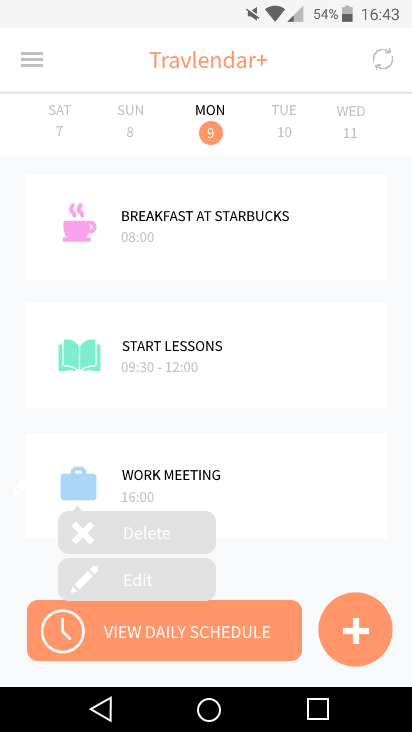
\includegraphics[width=0.50\textwidth]{Images/Mockup/BaseModificaDelete.png}}%
		\caption{Edit or delete appointment}
	\end{minipage}
	\begin{minipage}[b]{0.65\textwidth}
		\makebox[\textwidth][c]{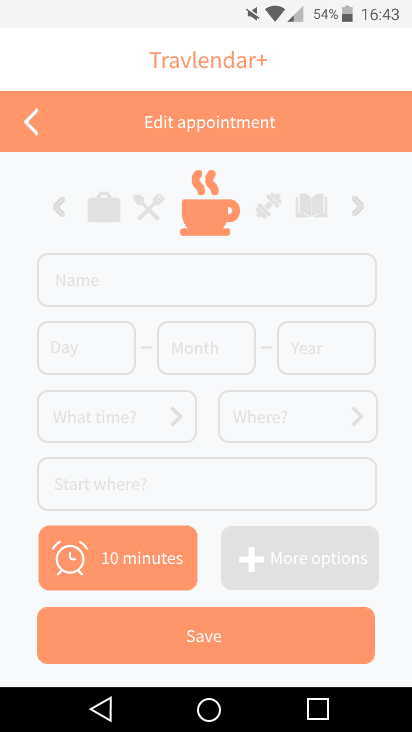
\includegraphics[width=0.50\textwidth]{Images/Mockup/EditAppointment.png}}%
		\caption{Edit appointment}
	\end{minipage}
\end{figure}
\clearpage
\begin{figure}[!h]
	\centering
	\begin{minipage}[b]{0.65\textwidth}
		\makebox[\textwidth][c]{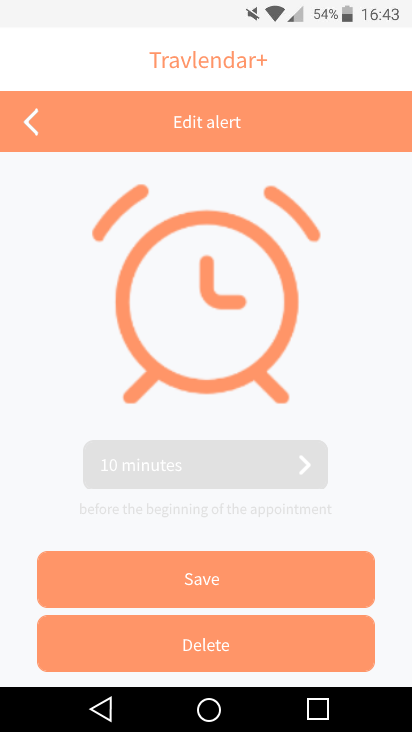
\includegraphics[width=0.50\textwidth]{Images/Mockup/AlarmEditDelete.png}}%
		\caption{Edit or delete alert}
	\end{minipage}
	\begin{minipage}[b]{0.65\textwidth}
		\makebox[\textwidth][c]{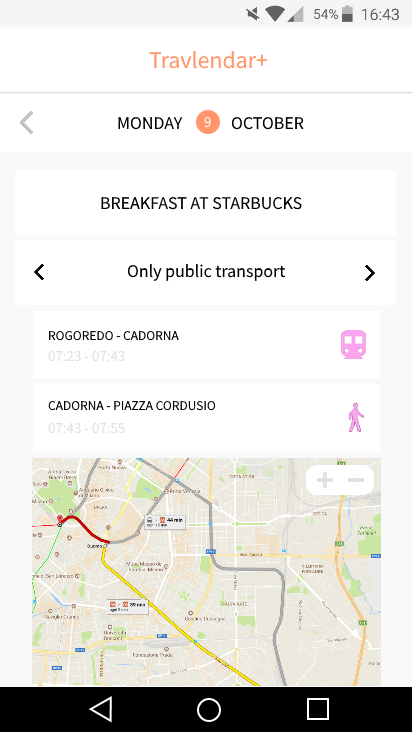
\includegraphics[width=0.50\textwidth]{Images/Mockup/TravelDetailsTrain.png}}%
		\caption{Travel details}
	\end{minipage}
\end{figure}
\clearpage
\begin{figure}[!h]
	\centering
	\begin{minipage}[b]{0.65\textwidth}
		\makebox[\textwidth][c]{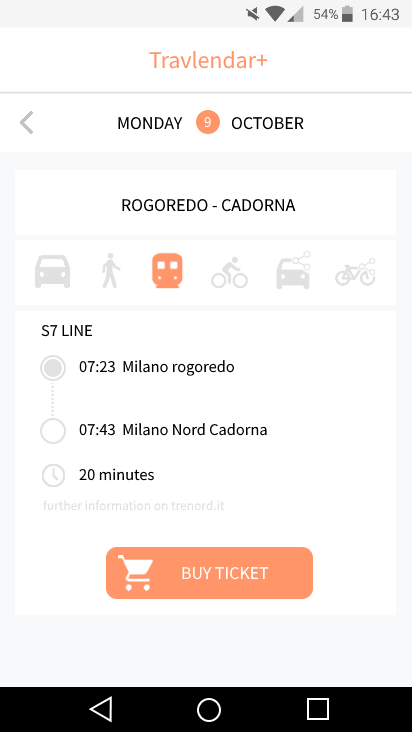
\includegraphics[width=0.50\textwidth]{Images/Mockup/MovementDetails.png}}%
		\caption{Movement details}
	\end{minipage}
\end{figure}

\subsubsection{Software interface}
The application makes uses of the following APIs:
\begin{itemize}
	\item Weather API: \href{url}{https://openweathermap.org/api}
	\item Google Maps API: \href{url}{https://developers.google.com/maps/}
	\item Trenord API: \href{url}{https://github.com/bluviolin/TrainMonitor/wiki/API-del-sistema-Viaggiatreno}
	\item Car2go API: \href{url}{https://github.com/car2go/openAPI}
	\item Enjoy API: \href{url}{https://github.com/mattiaongit/enjoy/blob/master/enjoy.py}
	\item BikeMi API: \href{url}{https://github.com/pierlauro/bikemi-unofficial-api}
	\item MoBike API: \href{url}{https://github.com/ubahnverleih/WoBike}
\end{itemize}
\clearpage
\subsection{Domain assumptions}
\begin{itemize}
	
\item \textbf{[D1]} The user is always connected via Internet and the connection is stable.
\item \textbf{[D2]} Information about weather, transport means, maps and travel times are provided by external APIs.
\item \textbf{[D3]} Data provided by external APIs are correct.
\item \textbf{[D4]} The process of ticket payment is made through an external public transport service.
\item \textbf{[D5]} If the payment is fulfilled without errors, the tickets are correctly received.

\end{itemize}

\subsection{Functional requirements}
\begin{itemize}
	\item \textbf{R1]} The user must be logged into the system to access application features.
	\item \textbf{[R2]} The user must be able to choose the option of creating a new appointment.
	\item \textbf{[R3]} The user must be able to choose the option of editing a selected appointment.
	\item \textbf{[R4]} The user must be able to choose the option of deleting a selected appointment.
	\item \textbf{[R5]} The system must be able to provide the user with an overview of his calendar and the user must be able to view all appointments fixed in a certain period.
	\item \textbf{[R6]} The user must be able to select a chosen day from the overview of his calendar.
	\item \textbf{[R7]} The user must be able to select a specific appointment in his calendar.
	\item \textbf{[R8]} The system must ask the user to provide all information needed for the creation of a new appointment, such as place and time of start and overall duration.
	\item \textbf{[R9]} The system must check if the information provided by the user are correct.
	\item \textbf{[R10]} The system must check if an appointment overlaps with other events and must eventually notify it to the user.
	\item \textbf{[R11]} The system must give the user access to all details of a selected appointment and the user must be allowed to edit the information needed.
	\item \textbf{[R12]} The user must be able to set advanced information for a created appointment.
	\item \textbf{[R13]} The user must be able to set an appointment as flexible, specifying the interval of time.
	\item \textbf{[R14]} The user must be able to set an appointment as repeatable, specifying the desired days.
	\item \textbf{[R15]} The system must schedule any flexible or repeatable appointment in the correct way, avoiding overlapping with other appointments.
	\item \textbf{[R16]} The appointment intended to be modified must have been previously successfully created and not already deleted.
	\item \textbf{[R17]} The user must confirm the creation of the new appointment.
	\item \textbf{[R18]} The user must confirm any appointment modification.
	\item \textbf{[R19]} The system must save the user modifications in memory and the calendar must be updated.
	\item \textbf{[R20]} The system must remove a deleted appointment from the memory and delete every alert related to it.
	\item \textbf{[R21]} The user must be able to switch between different possible calendar, such as daily calendar, weekly calendar and monthly calendar.
	\item \textbf{[R22]} The system must be able to provide information about the scheduled travels for a chosen day, showing the transport means and the estimated time required from each travel.
	\item \textbf{[R23]} The system must choose the best option between the possible travel alternatives according to the preferences expressed in the user profile settings and the information about external weather.
	\item \textbf{[R24]} The user must be able to select a specific travel in his daily schedule.
	\item \textbf{[R25]} The system must provide detailed information about the travels selected by the user, such as the trace route on the map and the weather conditions.
	\item \textbf{[R26]} The system must provide the user with an overview of the possible travel alternatives for the chosen travel, specifying all details for each one.
	\item \textbf{[R27]} The user must be able to filter the travel alternatives furnished by the system according to defined parameters, such as time of travelling or overall cost.
	\item \textbf{[R28]} The user must be able to choose a favourite travel option different from the displayed default one.
	\item \textbf{[R29]} The user must be able to select a specific movement in a travel.
	\item \textbf{[R30]} The system must provide detailed information about the movements selected by the user, such as the specific trace route on the map and the price of the ticket.
	\item \textbf{[R31]} The user must be able to choose an alternative transport mean for a selected movement, if there are any.
	\item \textbf{[R32]} The system must update the daily schedule according to the travel option chosen by the user and the user must be able to see the new updated schedule.
	\item \textbf{[R33]} The system must give to the user the possibility of buying the ticket for the selected travel.
	\item \textbf{[R34]} The system must save a copy of the bought tickets.
	\item \textbf{[R35]} The user must be able to access to a ticket page from the home page.
	\item \textbf{[R36]} The system must provide a list of all the bought tickets and the user must be able to select and view a specific one in full screen.
	\item \textbf{[R37]} The user must be able to access the preferences panel of his account.
	\item \textbf{[R38]} The system must give the user the possibility of setting various preferences, such as owned and preferred travel means, address of Home and other general travel preferences.
	\item \textbf{[R39]} The user must be able to edit the provided preferences when needed.
	\item \textbf{[R40]} The system must give the user the possibility of adding an alert to an appointment while it is being created or modified.
	\item \textbf{[R41]} The user must be able to choose a desired interval of time for the warning alert.
	\item \textbf{[R42]} The user must confirm the alert creation and the system must save the insertion in the memory.
	\item \textbf{[R43]} The user must be able to modify or remove the inserted alert when needed.
	\item \textbf{R44]} In case of any alert modification made by the user, the user must confirm the modification and the system must save all changes.
	
\end{itemize}

\subsection{Goals}
\subsubsection{[G1] Allow an User to create a new appointment in his calendar.}
\begin{itemize}
	\item \textbf{[R1]} The user must be logged into the system to access application features.
	\item \textbf{[R5]} The system must be able to provide the user with an overview of his calendar and the user must be able to view all appointments fixed in a certain period.
	\item \textbf{[R6]} The user must be able to select a chosen day from the overview of his calendar.
	\item \textbf{[R2]} The user must be able to choose the option of creating a new appointment.
	\item \textbf{[R8]} The system must ask the user to provide all information needed for the creation of a new appointment, such as place and time of start and overall duration.
	\item \textbf{[R40]} The system must give the user the possibility of adding an alert to an appointment while it is being created or modified.
	\item \textbf{[R9]} The system must check if the information provided by the user are correct.
	\item \textbf{[R12]} The user must be able to set advanced information for a created appointment.
	\item \textbf{[R10]} The system must check if an appointment overlaps with other events and must eventually notify it to the user.
	\item \textbf{[R17]} The user must confirm the creation of the new appointment.
	\item \textbf{[R19]} The system must save the user modifications in memory and the calendar must be updated.
\end{itemize}

\subsubsection{[G2] Allow a user to create flexible and repeatable appointments (such as lunches, study breaks etc.)}
\begin{itemize}
	\item \textbf{[R1]} The user must be logged into the system to access application features.
	\item \textbf{[R2]} The user must be able to choose the option of creating a new appointment.
	\item \textbf{[R12]} The user must be able to set advanced information for a created appointment.
	\item \textbf{[R13]} The user must be able to set an appointment as flexible, specifying the interval of time.
	\item \textbf{[R14]} The user must be able to set an appointment as repeatable, specifying the desired days.
	\item \textbf{[R15]} The system must schedule any flexible or repeatable appointment in the correct way, avoiding overlapping with other appointments.	
\end{itemize}

\subsubsection{[G3] Allow a user to edit an existing appointment in his calendar.}
\begin{itemize}
	\item \textbf{[R1]} The user must be logged into the system to access application features.
	\item \textbf{[R16]} The appointment intended to be modified must have been previously successfully created and not already deleted.
	\item \textbf{[R5]} The system must be able to provide the user with an overview of his calendar and the user must be able to view all appointments fixed in a certain period.
	\item \textbf{[R7]} The user must be able to select a specific appointment in his calendar.
	\item \textbf{[R3]} The user must be able to choose the option of editing a selected appointment.
	\item \textbf{[R11]} The system must give the user access to all details of a selected appointment and the user must be allowed to edit the information needed.
	\item \textbf{[R40]} The system must give the user the possibility of adding an alert to an appointment while it is being created or modified.
	\item \textbf{[R9]} The system must check if the information provided by the user are correct.
	\item \textbf{[R10]} The system must check if an appointment overlaps with other events and must eventually notify it to the user.
	\item \textbf{[R18]} The user must confirm any appointment modification.
	\item \textbf{[R19]} The system must save the user modifications in memory and the calendar must be updated.
\end{itemize}

\subsubsection{[G4] Allow a user to delete an existing appointment from his calendar.}
\begin{itemize}
	\item \textbf{[R1]} The user must be logged into the system to access application features.
	\item \textbf{[R5]} The system must be able to provide the user with an overview of his calendar and the user must be able to view all appointments fixed in a certain period.
	\item \textbf{[R16]} The appointment intended to be modified must have been previously successfully created and not already deleted.
	\item \textbf{[R7]} The user must be able to select a specific appointment in his calendar.
	\item \textbf{[R4]} The user must be able to choose the option of deleting a selected appointment.
	\item \textbf{[R18]} The user must confirm any appointment modification.
	\item \textbf{[R20]} The system must remove a deleted appointment from the memory and delete every alert related to it.
	\item \textbf{[R19]} The system must save the user modifications in memory and the calendar must be updated.	
\end{itemize}

\subsubsection{[G5] Allow a user to check his calendar to see his appointments.}
\begin{itemize}
	\item \textbf{[R1]} The user must be logged into the system to access application features. 
	\item \textbf{[R5]} The system must be able to provide the user with an overview of his calendar and the user must be able to view all appointments fixed in a certain period.
	\item \textbf{[R21]} The user must be able to switch between different possible calendar, such as daily calendar, weekly calendar and monthly calendar.
\end{itemize}

\subsubsection{[G6] Allow a user to view his Daily Schedule.}
\begin{itemize}
	\item \textbf{[R1]} The user must be logged into the system to access application features.
	\item \textbf{[R6]} The user must be able to select a chosen day from the overview of his calendar.
	\item \textbf{[R22]} The system must be able to provide information about the scheduled travels for a chosen day, showing the transport means and the estimated time required from each travel.
	\item \textbf{[R23]} The system must choose the best option between the possible travel alternatives according to the preferences expressed in the user profile settings and the information about external weather.
	\item \textbf{[D1]} The user is always connected via Internet and the connection is stable.
	\item \textbf{[D2]} Information about weather, transport means, maps and travel times are provided by external APIs.
	\item \textbf{[D3]} Data provided by external APIs are correct.
\end{itemize}

\subsubsection{[G7] Allow a user to see all the details of a specific travel.}
\begin{itemize}
	\item \textbf{[R1]} The user must be logged into the system to access application features.
	\item \textbf{[R22]} The system must be able to provide information about the scheduled travels for a chosen day, showing the transport means and the estimated time required from each travel.
	\item \textbf{[R24]} The user must be able to select a specific travel in his daily schedule.
	\item \textbf{[R25]} The system must provide detailed information about the travels selected by the user, such as the trace route on the map and the weather conditions.
	\item \textbf{[R29]} The user must be able to select a specific movement in a travel.
	\item \textbf{[R30]} The system must provide detailed information about the movements selected by the user, such as the specific trace route on the map and the price of the ticket.
	\item \textbf{[D1]} The user is always connected via Internet and the connection is stable.
	\item \textbf{[D2]} Information about weather, transport means, maps and travel times are provided by external APIs.
	\item \textbf{[D3]} Data provided by external APIs are correct.
\end{itemize}

\subsubsection{[G8] Allow a user to navigate and choose between different travel alternatives.}
\begin{itemize}
	\item \textbf{[R1]} The user must be logged into the system to access application features. 
	\item \textbf{[R24]} The user must be able to select a specific travel in his daily schedule.
	\item \textbf{[R26]} The system must provide the user with an overview of the possible travel alternatives for the chosen travel, specifying all details for each one.
	\item \textbf{[R27]} The user must be able to filter the travel alternatives furnished by the system according to defined parameters, such as time of travelling or overall cost.
	\item \textbf{[R28]} The user must be able to choose a favourite travel option different from the displayed default one.
	\item \textbf{[R29]} The user must be able to select a specific movement in a travel.
	\item \textbf{[R31]} The user must be able to choose an alternative transport mean for a selected movement, if there are any.
	\item \textbf{[R32]} The system must update the daily schedule according to the travel option chosen by the user and the user must be able to see the new updated schedule.
	\item \textbf{[D1]} The user is always connected via Internet and the connection is stable.
	\item \textbf{[D2]} Information about weather, transport means, maps and travel times are provided by external APIs.
	\item \textbf{[D3]} Data provided by external APIs are correct.
\end{itemize}

\subsubsection{[G9] Allow a user to manage alerts for each appointment.}
\begin{itemize}
	\item \textbf{[R40]} The system must give the user the possibility of adding an alert to an appointment while it is being created or modified.
	\item \textbf{[R41]} The user must be able to choose a desired interval of time for the warning alert.
	\item \textbf{[R42]} The user must confirm the alert creation and the system must save the insertion in the memory.
	\item \textbf{[R43]} The user must be able to modify or remove the inserted alert when needed.
	\item \textbf{[R44]} In case of any alert modification made by the user, the user must confirm the modification and the system must save all changes.
\end{itemize}

\subsubsection{[G10] Allow a user to manage his travel preferences.}
\begin{itemize}
	\item \textbf{[R37]} The user must be able to access the preferences panel of his account from the home page.
	\item \textbf{[R38]} The system must give the user the possibility of setting various preferences, such as owned and preferred travel means, address of Home and other general travel preferences.
	\item \textbf{[R39]} The user must be able to edit the provided preferences when needed.	
\end{itemize}

\subsubsection{[G11] Allow a user to buy public transportation tickets.}
\begin{itemize}
	\item \textbf{[R1]} The user must be logged into the system to access application features.
	\item \textbf{[R29]} The user must be able to select a specific movement in a travel.
	\item \textbf{[R33]} The system must give to the user the possibility of buying the ticket for the selected travel.
	\item \textbf{[R34]} The system must save a copy of the bought tickets.
	\item \textbf{[D5]} The payment process and ticket acquisition is made by an external public transport service.
	\item \textbf{[D1]} The user is always connected via Internet and the connection is stable.
	\item \textbf{[D4]} The process of ticket payment is made through an external public transport service.
	\item \textbf{[D5]} If the payment is fulfilled without errors, the tickets are correctly received.
\end{itemize}

\subsubsection{[G12] Allow a user to view the previously bought tickets.}
\begin{itemize}
	\item \textbf{[R1]} The user must be logged into the system to access application features.
	\item \textbf{[R34]} The system must save a copy of the bought tickets.
	\item \textbf{[R35]} The user must be able to access to a ticket page from the home page.
	\item \textbf{[R36]} The system must provide a list of all the bought tickets and the user must be able to select and view a specific one in full screen.	
\end{itemize}

\subsection{Design constraints}
\subsubsection{Standards compliance}
The application must require to the user different permissions:
\begin{itemize}
	\item Access to the calendar;
	\item Get hit position with GPS;
	\item Access to device storage.
\end{itemize}
\subsubsection{Hardware limitations}
The application, at the moment, runs only on Android 4.0.3 version or newer. \\
The device needs:
\begin{itemize}
	\item Internet connection;
	\item GPS;
	\item Space for save application in memory.
\end{itemize}
Actual devices on the market satisfy all these requirements.
\subsection{Software system attributes}
\subsubsection{Reliability}
The system must guarantee a 24/7 service.
\subsubsection{Availability}
The system requires a GPS service and internet connection in order to work properly. When the connection is down the system works with the last updated information available in the device memory.  
\subsubsection{Security}
The application must provide secure storage for all sensitive data inserted by the user. One way to achieve it is the use of cryptographical techniques.
\subsubsection{Maintainability}
The application will be released in beta version, meaning that it may eventually have some bugs. The application will be periodically upgraded and each release will be focus on solving detected problems.
Periodically all information stored in the application must be backed up, in order to reduce the possibility of losing information in case of malfunctions.
\subsubsection{Portability}
The application will be released only for Android smartphones (more specifically only for Android version 4.0.3 Ice Cream Sandwich or later).\\
Future plan is to lead the software also on iOS devices.

